\lecture{20}{28. April 2025}{Corrosion and Degradation of Materials}

\section{Corrosion and Degradation of Materials}

\subsection{Introduction}
Most materials experience some type of interaction with most environments. Often, such interactions impair a material's usefulness as a result of the deterioration of its mechanical properties, physical properties, or appearance.

The mechanisms behind deterioration is different for the three material types. In metals, there is actual material loss either by dissolution (\textit{corrosion}) or by the formation of a nonmetallic scale or film (\textit{oxidation}). Ceramic materials are relatively resistant to deteriration, which usually only occurs in extreme environments -- this process is also frequently called \textit{corrosion}. For polymers, mechanisms and consequences differ from those for metals and ceramics, and the term \textit{degradation} is most frequently used. 

\begin{definition}[Corrosion]
  Corrosion is defined as the destructive and unintentional attack on a metal; it is electrochemical and begins at the surface.
\end{definition}

\subsection{Electrochemical considerations}
For metallic materials, the corrosion process is normally electrochemical, i.e. an oxidation reaction. A hypothetical metal M that has a valence of $n$ (or $n$ valence electrons) may experience oxidation according to the reaction:
\[ 
M \rightarrow M^{n+} + ne^{-}
\]
in which $M$ becomes an $n+$ positively charged ion and in the process loses its $n$ valence electrons. 

The electrons generated from each metal atom that is oxidized must be transferred to and become part of another chemical species in what is termed a \textit{reduction} reaction. E.g. some metals undergo corrosion in acid solutions, which have a high concentration of $H^{+}$ ions. These are reduced as follows:
\[ 
2H^{+} + 2e^{-} \rightarrow H_2
.\]
Other reactions are also possible. If the acid solutions has dissolved oxygen water might be formed instead of hydrogen gas, as least to some degree and so on. Similarly, any metal ions present in the solution may also be reduced. For ions that can exist in more than one valence state (multivalent ions), reduction may occur as:
\[ 
M^{n+} + e^{-} \rightarrow M^{(n-1)+}
.\]

An overall electrochemical reaction must consist of at least one oxidation and one reduction reaction and will be their sums. This is called a \textit{redox}-reaction and the individual \textit{oxidation} and \textit{reduction}-reactions are called \textit{half-reactions}.

\subsubsection{Electrode potentials}

\begin{figure} [ht]
  \centering
  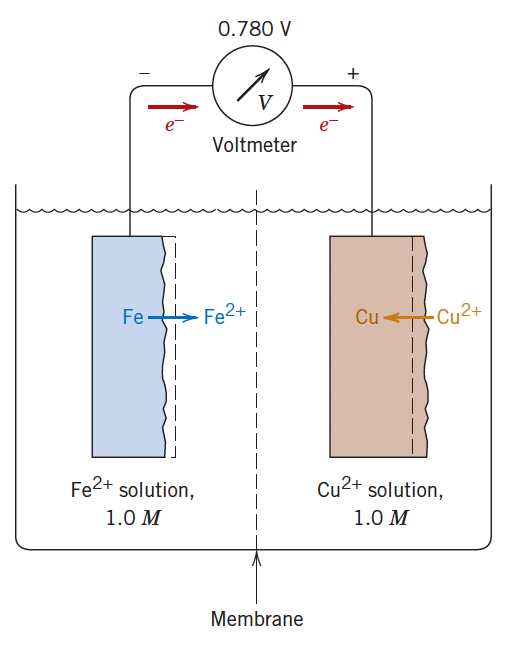
\includegraphics[width=0.5\linewidth]{./figures/f20_1.png}
  \caption{An electrochemical cell consisting of iron and copper electrodes.}
  \label{fig:f20_1}
\end{figure}

On the left hand side of \textbf{\autoref{fig:f20_1}} is a piece of pure iron immersed in a solution of $\mathrm{Fe}^{2+}$ ions of \qty{1}{M} concentration. The other side similarly contains a pure copper piece immersed in a solution of copper ions. If the iron and copper electrodes are connected electrically, reduction will occur for the copper and the iron will be oxidized as follows:
\[ 
\mathrm{Cu}^{2+} + \mathrm{Fe} \rightarrow \mathrm{Cu} + \mathrm{Fe}^{2+}
.\]
Here $\mathrm{Cu}^{2+}$ ions deposit as metallic copper on the copper electrode, whereas iron dissolves (corrodes) on the other side and go into solution as $\mathrm{Fe}^{2+}$ ions. 

When a net current passes through the external circuit, electrons generated from the oxidation of iron flow to the copper cell in order to reduce the $\mathrm{Cu}^{2+}$. In addition, there will be some net ion motion from each cell to the other across the membrane. This is called a \textit{galvanic couple}.

An electric potential or voltage exists between the two cell halves, and its magnitude can be determined by connecting a voltmeter. A potential of \qty{0,78}{V}  results for a copper-iron galvanic cell when the temperature is \qty{25}{\celsius}. 

Various electrode pairs have different voltages (e.g. a iron-zinc cell has an associated potential of \qty{0,323}{V}. The magnitude of this voltage may be thought of as the driving force of the redox reaction. 

\subsubsection{The standard EMF series}
These meassured cell voltages represent only differences in electrical potential, and thus it is convenient to establish a reference point, or reference cell to which other cell halves may be compared. This reference point has been chosen to be hydrogen ions being reduced to hydrogen gas in the presense of a platinum catalyst.

Based on this, the \textit{electromotive force series} shown on \textbf{\autoref{fig:f20_2}} can be generated. This shows the corrosion tendencies of the metals. The ones at the top are \textit{noble} or chemically inert and as one moves down the table the metals become increasingly more active.
\begin{figure} [ht]
  \centering
  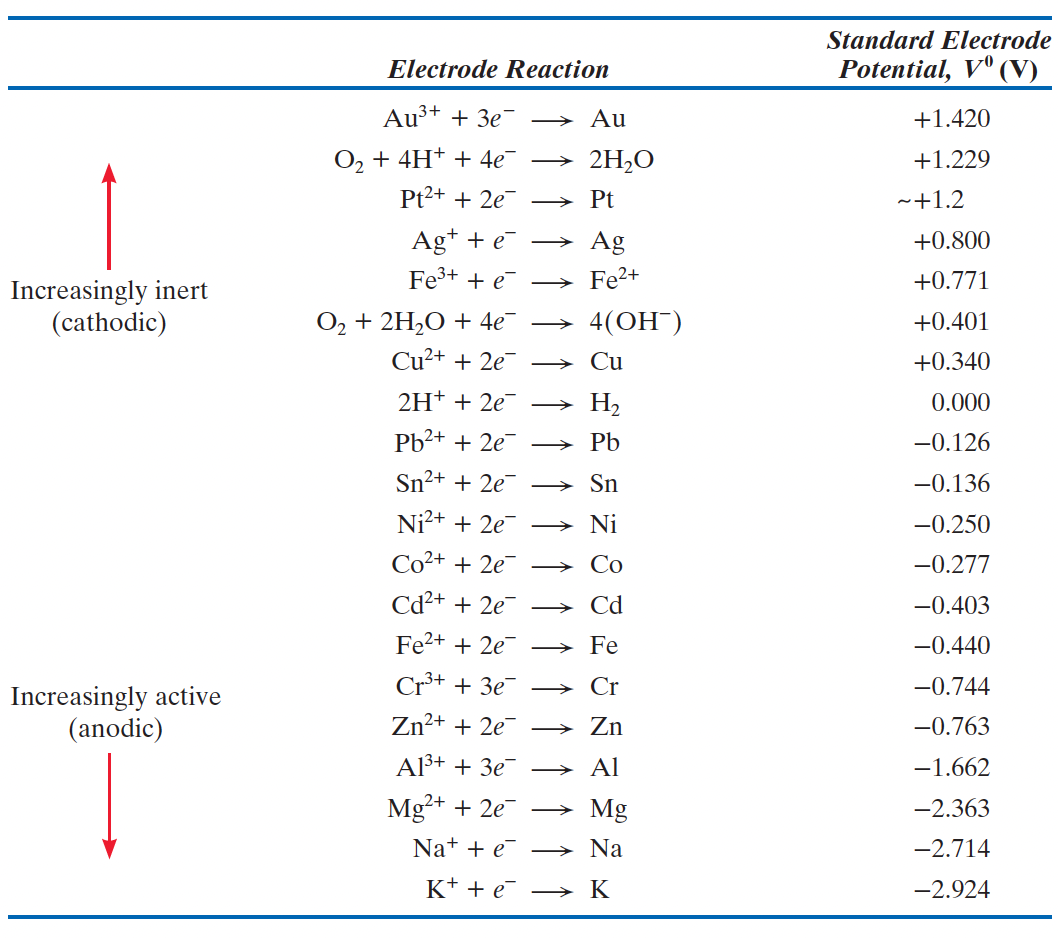
\includegraphics[width=0.5\linewidth]{./figures/f20_2.png}
  \caption{EMF series}
  \label{fig:f20_2}
\end{figure}

The numbers shown on \textbf{\autoref{fig:f20_2}} are for the reduction reactions. For the corresponding oxidation reactions the sign of the voltage must be flipped.

Let $V_2^{0}$ be the cell potential for the reduction half cell and let $V_1^{0}$ be the cell potential (with flipped sign) for the oxidation reaction. Then the overall cell potential $\Delta V^{0}$ can be calculated as:
\[ 
\Delta V^{0} = V_2^{0} - V_1^{0}
.\]
For this reaction to occur spontaneously, $\Delta V^{0}$ must be positive.

\subsubsection{Influence of concentration and temperature on cell potential}
The EMF series shown on \textbf{\autoref{fig:f20_2}} only applies to highly idealized electrochemical cells. Altering temperature or solution concentrations or using alloy electrodes instead of pure metals changes the cell potential, and in some cases, the spontaneous reaction direction may be reversed. 

Let $M_1$ and $M_2$ be electrodes of pure metals, the cell potential depends on the absolute temperature $T$ and the molar ion concentrations $\left[ M_1^{n+} \right]$ and $\left[ M_2^{n+} \right]$ according to the Nernst equation:
\[ 
\Delta V = \left( V_2^{0} - V_1^{0} \right) - \frac{RT}{n \mathcal{F}} \ln \frac{\left[ M_1^{n+} \right]}{\left[ M_2^{n+} \right]}
\]
where $\mathcal{F}$ is the Faraday constant. 

\subsubsection{The Galvanic series}
Even though \textbf{\autoref{fig:f20_2}} is highly idealized it nonetheless indicates the relative reactivities of the metals. A more realistic and practical ranking is provided by the \textit{Galvanic series} on \textbf{\autoref{fig:f20_3}}.
\begin{figure} [ht]
  \centering
  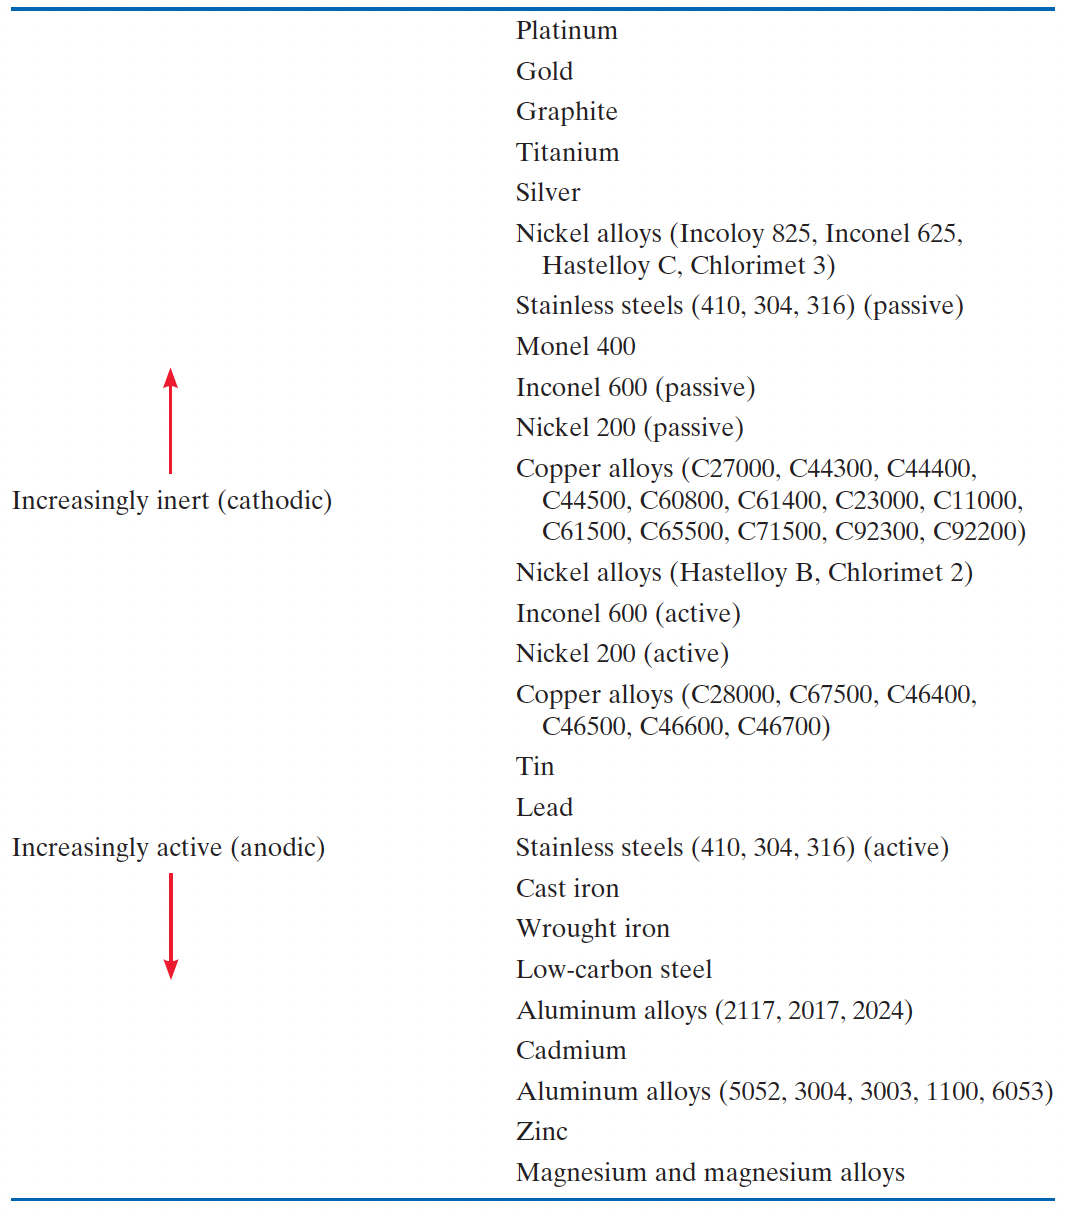
\includegraphics[width=0.5\linewidth]{./figures/f20_3.png}
  \caption{Galvanic series}
  \label{fig:f20_3}
\end{figure}

\subsection{Corrosion Rates}
The half-cell potentials listed until now have assumed that the systems are at equilibrium. I.e. it has been assumed that there is no current flow through the external circuit. Real corroding systems are not at equilibrium; there is a flow of electrons from anode to cathode, which means that the previously introduced half-cell potentials cannot be applied.

Furthermore, these half-cell potentials represent the magnitude of the driving force, or the tendency for a particular reaction to take place. However, although these potentials may be used to determine spontaneous reaction directions they provide no information on corrosion rates.

The corrosion rate, or the rate of material removal as a consequence of the chemical action, is an important corrosion parameter. This may be expressed as the \textit{corrosion penetration rate} (CPR), ir the thickness loss of material per unit of time. The formula for this is:
\[ 
\mathrm{CPR} = \frac{KW}{\rho A t}
\]
where $W$ is the weight loss after exposure time $t$, $\rho$ and $A$ represent the density and exposed specimen area, respectively, and $K$ is a constant. For the CPR to be expressed in milimeters per year \unit{mm / yr}, $K = \num{87,6}$, if one expresses weight in \unit{mg}, density in \unit{g / cm^3}, area in \unit{cm^2} and time in \unit{h}.

Because there is an electric current associated with electrochemical reactions, we can also express the corrosion rate in terms of this current, or more specifically the current density, $i$. The rate $r$ in units of \unit{mol/\m^2.\s}, is determined using the expression:
\[ 
r = \frac{i}{n \mathcal{F}}
.\]

\subsection{Prediction of Corrosion Rates}

\subsubsection{Polarization}
\begin{figure} [ht]
  \centering
  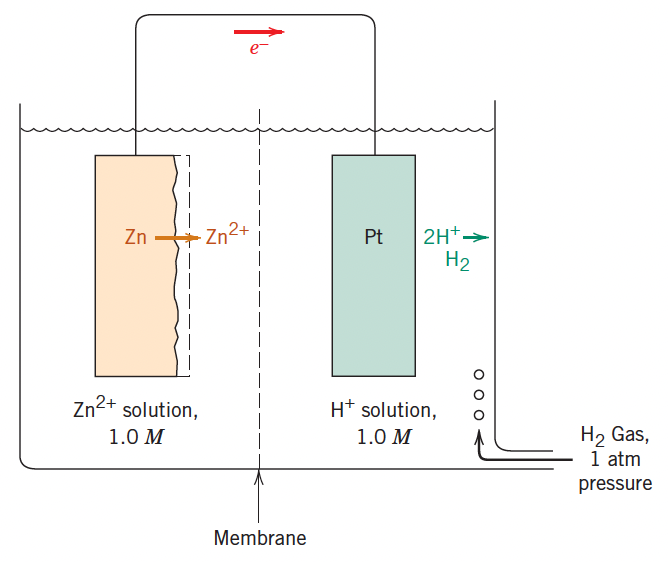
\includegraphics[width=0.5\linewidth]{./figures/f20_4.png}
  \caption{Electrochemical cell of Zinc and hydrogen that has been short-circuited}
  \label{fig:f20_4}
\end{figure}
If we consider the standard $\mathrm{Zn}$/$\mathrm{H}_2$ electrochemical cell shown on \textbf{\autoref{fig:f20_4}} the potential of the two electrodes are not the same as shown on \textbf{\autoref{fig:f20_1}} because the system is not at equilibrium. The displacement of each electrode potential from its equilibrium value is termed \textit{polarization}, and the magnitude of this displacement is the \textit{overvoltage}, normally represented by $\eta$. Overvoltage is expressed in terms of plus or minus volts relative to the equilibrium potential. For example, suppose that the zinc electrode in \textbf{\autoref{fig:f20_4}} has a potential of $-\qty{0,621}{V}$ after it has been connected to the platinum electrode. The equilibrium potential is $-\qty{0,763}{V}$ and therefore:
\[ 
\eta = -\qty{0,621}{V}  - \left( - \qty{0,763}{V}  \right)= \qty{0,142}{V} 
.\]

There are two types of polarization -- activation and concentration. 

\paragraph{Activation Polarization} All electrochemical reactions consist of a sequence of steps that occur in series at the interface between the electrode and the solution. \textit{Activation polarization} refers to the condition in which the reaction rate is controlled by the one step in the series that occurs at the slowest rate. The term \textit{activation} is applied to this type of polarization, because an activation energy barrier is associated with this slowest, rate-limiting step.

For activation polarization, the relationship between overvoltage $\eta_a$ and current density $i$ is:
\[ 
\eta_a = \pm \beta  \log \frac{i}{i_0}
\]
where $\beta$ and $i_0$ are constants for the particular half-cell. The parameter $i_0$ is called the \textit{exchange current density}. Equilibrium for some particular half-cell reaction is really a dynamic state on the atomic level -- i.e. oxidation and reduction keep occuring but at some point they occur at the same rate so that there is no net reaction. The exhange current density is the current density at equilibrium or:
\[ 
r_{\mathrm{red}} = r_{\mathrm{oxid}} = \frac{i_0}{n \mathcal{F}}
.\]
Use of the term, \textit{current density} for $i_0$ is a little misleading inasmuch as there is no net current. $i_0$ is determined experimentally and varies from system to system.

\paragraph{Concentration Polarization} exists when the reaction rate is limited by diffusion in the solution. At high reaction rates or low solute concentrations, a depletion zone may be formed in the vicinity of the interface between the electrode and the solution, because the ions are not being replenished at an adequate pace. Thus diffusion of ions to the interface is rate controlling and the system is said to be concentration polarized.

The mathematical expression relating concentration polarization overvoltage $\eta_c$ and current density $i$ is:
\[ 
\eta_c = \frac{\num{2,3} RT}{n \mathcal{F}} \log \left( 1 - \frac{i}{i_L} \right)
\]
here $i_l$ is the limiting diffusion current density. 

\subsection{Passivity}
Under particular conditions, some normally active metals and alloys lose their chemical reactivity. This phenomenon, called \textit{passivity}, is displayed by chromium, iron, nickel, titanium and many of their alloys. It is believed that this happens as a thin oxide film on the metal surface, which serves as a protective barrier to further corrosion. Passivation is also the reason stainless steels are so resistant to oxidation. Theese contain at least 11\% chromium, which acts as a solid-solution alloying element and minimizes the formation of rust. Aluminium also passivates.

Some metals passivate more readily than others and for some metals that are slow to form the protective oxidation layer corrosion rates may be boosted by as much as \num{100000} times of the oxidation layer is broken.


\subsection{Environmental Effects}
The environmental variables which include fluid velocity, temperature and composition, can have a decided influence on the corrosion properties of the materials that are in contact with it. In most instances, increasing fluid velocity enhances the rate of corrosion due to erosive effects. The rates for most chemical reactions (including corrosion reactions) increase for temperature and the concentration of corrosive species such as $H^{+}$ ions also increases corrosion rates.

Cold working a ductile metal increases its strength, but a cold-worked metal is more susceptible to corrosion than an annealed version of the same metal. Therefore one should carefully consider using cold-working in corrosive environments.


\subsection{Forms of Corrosion}
Often it is convenient, to classify corrosion according to the manner in which it manifests. Metallic corrosion is sometimes classified into eight forms: \textit{uniform}, \textit{galvanic}, \textit{crevice}, \textit{pitting}, \textit{intergranular}, \textit{selective leaching}, \textit{erosion-corrosion}, and \textit{stress corossion}. Also the topic of Hyrogen embrittlement is presented, in a strict sense this is a type of failure rather than a form of corrosion, however, it is often a result of hydrogen produced during corrosion.

\subsubsection{Uniform attack}
Uniform attack is a form of electrochemical corrosion that occurs with equivalent intensity over the entire exposed surface and often leaves behind a scale or deposit. In a microscopic sense, the oxidation and reduction reactions occur randomly over the entire surface. Familiar examples include general rusring of steel and iron and tarnishing of silverware. This is the most common form of corrosion and it can relatively easily be predicted.

\subsubsection{Galvanic corrosion}
Galvanic corrosion occurs when two metals or alloys having different compositions are elctrically coupled while exposed to an electrolyte. The less noble or more reactive of the metals experiences corrosion and the more inert metal is protected. As examples, steel screws corrode when in contact with brass in a marine environment, and if copper and steel tubing are joined in a domestic water heater, the steel corrodes in the vicinity of the junction. 

The galvanic series on \textbf{\autoref{fig:f20_2}} indiated the relative reactivities in seawater of various metals and alloys. When two alloys are coupled in seawater, the one lower in the series experiences corrosion. It is also worth noting from this series that some alloys are listed twice (e.g. nickel and the stainless steels), in both active and passive states. 

A number of measures may be taken to reduce the effects of galvanic corrosion significantly, including:
\begin{itemize}
  \item If coupling of dissimilar metals is necessary, choose two metals that are close in the galvanic series
  \item Avoid an unfavourable anode-to-cathode surface area ratio; use an anode area as large as possible
  \item Electrically insulate dissimilar metals from each other
  \item Electrically connect a third, anodic metal to the other two; this is a form of cathodic protection, discussed in \textbf{\autoref{afs:cathodic}}
\end{itemize}

\subsubsection{Crevice corrosion}
Electrochemical corrosion may also occur as a consequence of concentration differences of ions or dissolved gases in the electrolyte solution and between two regions of the same metal piece. For such a \textit{concentration cell}, corrosion occurs in the locale that has the lower concentration. A good example of this type of corrosion occurs in the crevices and recesses or under deposits of dirt or corrosion products where the solution becomes stagnant and there is localized depletion of dissolved oxygen. Corrosion preferentially occurring at these positions is called \textit{crevice corrosion} and is shown on \textbf{\autoref{fig:f20_5}}. The crevice must be wide enough for the solution to penetrate yet narrow enough for stagnancy: usually the width is several thousands of a millimeter.

\begin{figure} [ht]
  \centering
  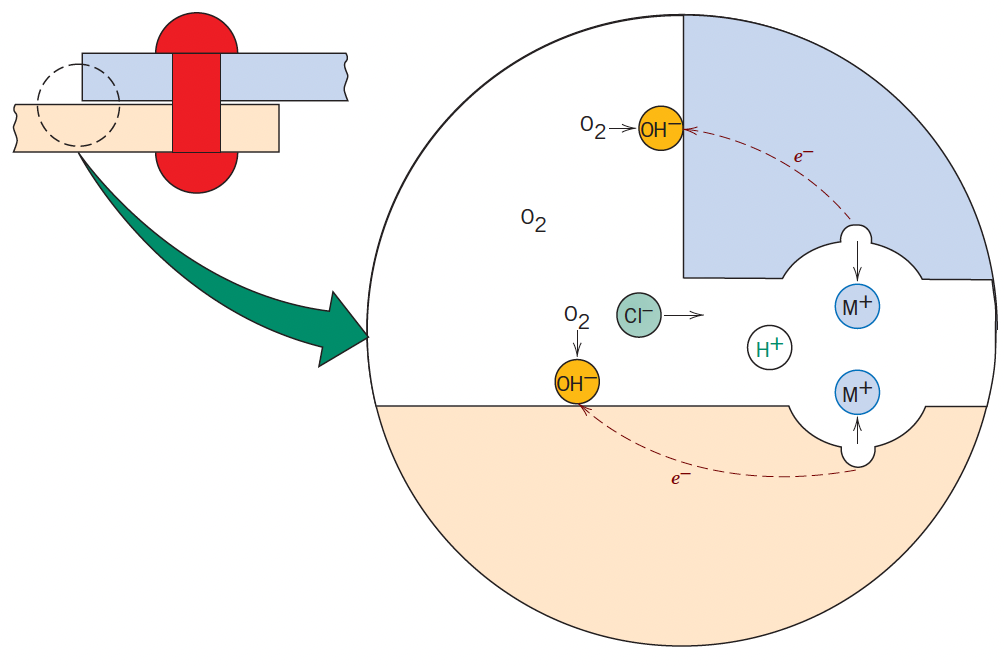
\includegraphics[width=0.5\linewidth]{./figures/f20_5.png}
  \caption{Crevice corrosion between two riveted sheets.}
  \label{fig:f20_5}
\end{figure}

The proposed mechanism for crevice corrosion is illustrated in \textbf{\autoref{fig:f20_5}}. After oxygen has been depleted within the crevice, oxidation of the metal occurs at this position. Electrons from this electrochemical reaction are conducted through the metal to adjacent external regions, where they are consumed by reduction. 

In many aqueous environments, the solution within the crevice has been found to develop high concentrations of $\mathrm{H}^{+}$ and $\mathrm{Cl}^{-}$ ions.

Crevice corrosion may be prevented by welding instead of riveting or bolting joints, and generally trying to avoid stagnant areas as much as possible.

\subsubsection{Pitting}
Pitting is another form of very localized corrosion attack in which small pits or holes form. They ordinarily penetrate from the top of a horizontal surface downward in a nearly vertical direction. Often pitting has very little material loss and goes undetected until failure.

The mechanism in pitting is probably the same as for crevice corrosion, in that oxidation occurs within the pit iself, with complementary reduction at the surface. It is supposed that gravity causes the pits to grow downward, the solution at the pit tip becoming more concentrated and dense as the pit grows. A pit may be initiated by a localized surface defect. In fact, it has been observed that polished specimens undergo less pitting than non-polished specimens.

\subsubsection{Intergranular corrosion}
As the name suggests, intergranular corrosion occurs preferentially along grain boundaries for some alloys and in specific environments. The net result is that a macroscopic specimen disintegrates along its grain boundaries. This type of corrosion is prevalent in some stainless steels. When heated to temperatures between \qty{500}{\celsius} and \qty{800}{\celsius} for sufficiently long time periods, these alloys become sensitized to intergranular attack. It is believed that this heat treatment permits the formation of small precipitate particles of chromium carbide $\mathrm{Cr}_{23}\mathrm{C}_6$. These particles form along the grain boundaries. Both the chromium and carbon must diffuse to the grain boundaries to form the precipitates, which leaves achromium-depleted zone adjacent to the grain boundary. Consequentially, this grain boundary region is now highly susceptible to corrosion.

Intergranular corrosion is an especially severe problem in the welding of stainless steels when it is called \textit{weld decay}. 

\subsubsection{Selective leaching}
Selective leaching is found in solid solution alloys and occurs when one element or constituent is preferentially removed as a consequence of corrosion processes. The most common example is the dezincification of brass, in which zinc is selectively leached from a copper-zinc brass alloy. The mechanical properties of the alloy are significantly impaired because only a porous mass of copper remains in the region that has been dezincified.

\subsubsection{Erosion-corrosion}
Erosion-corrosion arises from the combined action of chemical attack and mechanical abrasion or wear as a consequence of fluid motion. Virtually all metal alloys are susceptible to erosion-corrosion to some degree. It is especially harmful to alloys that passivate: the abrasive action may erode away the passivation film exposing the bare metal surface. If a new protective layer is not formed quickly enough the erosion may be severe. 

Erosion-corrosion is commonly found in piping, especially at bends, elbows and abrupt changes in pipe diameter.

\subsubsection{Stress corrosion}
Stress corrosion results from the combined action of an applied tensile stress and a corrosive environment. Some materials are virtually inert in a particular corrosive medium, but become susceptible to attack once a stress is applied. Small cracks form and then propagate in a direction perpendicular to the stress. Failure behaviour is characteristic of that for a brittle material, even though the metal alloy is intrinsically ductile.


\subsubsection{Hydrogen emrittlement}
Various metal alloys, speficially some steels, experience a significant reduction in ductility and tensile strength when atomic hydrogen penetrates into the material.

This phenomenon is called \textit{hydrogen embrittlement}. Hydrogen in its molecular form diffuses interstitially through the crystal lattice and concentrations as low as several ppm can lead to cracking. Hydrogen embrittlement is similar to stress corrosion in that a normally ductile metal experiences brittle fracture.


\subsection{Corrosion Environments}
Corrosive environments include the atmosphere, aqueous solutions, soils, acids, bases, inorganic solvents, molten salts, liquid metals and the human body. On a tonnage basis, atmospheric corrosion accounts for the greatest losses.

Water environments can have a variety of compositions and corrosion characteristics. Freshwater normally contains dissolved oxygen as well as minerals. Seawater contains approximately \num{3,5} \% salt. Seawater is generally more corrosive than freshwater, frequently producing pitting and crevice corrosion. 

Soils have a wide range of compositions and susceptibilities to corrosion. Compositional variables include moisture, oxygen, salt content, alkalinity and acidity as well as the presense of various forms of bacteria.


\subsection{Corrosion prevention} 
Perhaps the most common and easiest way of preventing corrosion is through the judicious selection of materials once the corrosion environment has been defined.

Changing the character of the environment, if possible, may also significantly influence corrosion. Lowering the fluid temperature and/or velocity usually produces a reduction in the rate at which corrosion occurs. Often, increasing or decreasing the concentration of some species in the solution will have a positive effect.

Inhibitors are substances that, when added in relatively low concentration to the environment, decrease its corrosiveness. The specific inhibitors one can use depends on the alloys and environments one is working with. 

Physical barriers to corrosion can also be applied to surfaces in the form of films or coatings. Here a large array of products are available.

\subsubsection{Cathodic protection} \label{afs:cathodic}
One of the most effective means of corrosion prevention is \textit{cathodic protection}. It simply involves supplying, from an external source, electrons to the metal to be protected, making it a cathode.

One cathodic protection technique employs a galvanic couple. By coupling the metal to be protected with a more reactive metal the more reactive metal ``sacrifices'' itself and corrodes whilst protecting the lesser reactive metal.

The process of \textit{galvanizing} is simply one in which a layer of zinc if applied to the surface of steel by hot dipping. Zinc is anodic and will thus cathodiaclly protect the steel. 

The electrons can also be supplied with an external DC power source. 

\subsection{Oxidation}

\subsubsection{Mechanisms}
The process of oxide layer formation is an electrochemical one, which may be expressed as:
\[ 
M + \frac{1}{2} \mathrm{O}_2 \rightarrow \mathrm{MO}
.\]
For the oxide layer to increase in thickness it is necessary that electrons be conducted to the scale-gas interface, at which point the reduction reaction occurs. Thus, the oxide scale serves both as an electrolyte through which ions diffuse and as an electrical circuit for the passage of electrons.


\subsubsection{Scale types}
The Pilling-Bedworth ratio is a name for the ratio of the relative volumes of oxide and metal. It can be determined as:
\[ 
\text{P-B ratio} = \frac{A_{O} \rho_M}{A_M \rho_O}
\]
where $A_O$ is the molecular weight of the oxide, $A_M$ is the molecular weight of the metal, and $\rho_O$ and $\rho_M$ are the oxide and metal densities, respectively. 

For metals with a P-B ratio less than unity, the oxide film tends to be porous and unprotective because it is insufficient to cover the entire surface. If the ratio is greater than unity, compressive stresses result in the film as it forms. For a ratio greater than 2 to 3, the oxide coating may crack and flake off, continually exposing a fresh and unprotected metal surface. The ideal P-B ratio for the formation of a protective oxide coating is unity. Whereas unprotective ones form for P-B ratios less than unity or greater than about 2. 


\subsubsection{Kinetics}
One of the primary concerns relative to metal oxidation is the rate at which the reaction progresses. Because the oxide scales usually remains on the surface, the rate of reaction may be determined by meassuring the weight gain per unit area as a function of time.

When the oxide that forms is nonporous and adheres to the metal surface, the rate of layer growth is controlled by ionic diffusion. A parabolic relationship exists between weight gain per unit area $W$ and the time $t$ as follows:
\[ 
W^2 = K_1 t + K_2
\]
where $K_1$ and $K_2$ are time-independent constants at a given temperature.

In the oxidation of metals for which the scale is porous or flakes off (i.e. for P-B ratios less than about 1 or greater than about 2), the oxidation rate expression is linear, as:
\[ 
W = K_3 t
\]
where $K_3$ is a constant.

A third reaction rate law has been observed for very thin oxide layers (generally less than \qty{100}{nm}) that form at relatively low temperatures. The dependence of weight gain on time is logarithmic and takes the form:
\[ 
W = K_4 \log \left( K_5 t + K_6 \right)
.\]

\subsubsection{Corrosion of ceramic materials}
Ceramic materials, being compounds between metallic and nonmetallic elements, may be though of as being corrosion products. Thus, they are exceedingly immune to corrosion by almost all environments, especially at room temperature.


\subsubsection{Degradation of polymers}
Polymeric materials also experience deterioration by means of environmental interactions. However, an undesirable interaction is here called degradation rather than corrosion because the processes are dissimilar at the basic level. Polymeric degradation is not electrochemical but instead physiochemical in nature. 


\subsection{Swelling and Dissolution}
When polymers are exposed to liquids, the main forms of degradation are swelling and dissolution. With swelling, the liquid or solute diffuses into and is absorbed within the polymer, the small solute molecules fit into and occupy positions among the polymer molecules. This forces apart the macromolecules such that the specimen expands or swells. The increase in chain separation leads to a reduction in the secondary intermolecular bonding forces, which in turns softens the polymer and makes it more ductile. 

Swelling may be considered a partial dissolution process in which there is only limited solubility of the polymer in the solvent. Dissolution, which occurs when the polymer is completely soluble, may be thought of as a continuation of swelling. As a rule of thumb, the greater the similarity of chemical structure between the solvent and polymer, the greater the likelihood of swelling and/or dissolution. For example, many hydrocarbon rubbers readily absorb hydrocarbon liquids such as gasoline, but absorb virtually no water.

Swelling and dissolution traits also are affected by temperature, as well as by the characteristics of the molecular structure. In general, increasing molecular weight, increasing degree of crosslinking and crystallinity, and decreasing temperature result in a reduction of these deteriorative processes.

\subsection{Bond Rupture}
Polymers may also experience degradation by a process termes \textit{scission} -- the severance or rupture of molecular chain bonds. This changes the chain lengths and in turn the properties of the polymer.


\subsubsection{Radiation effects}
Certain types of radiation posesses sufficient energy to penetrate a polymer specimen and interact with the constituent atoms or their electrons. One such reaction is \textit{ionization}, in which the radiation removes an orbital electron from a specific atom converting it into an ion. As a consequence one of the covalent bonds associated with the atom is broken and there is a rearrangement of atoms at that point.

\subsubsection{Chemical reaction effects}
Oxygen, ozone and other substances can cause or accelerate chain scission as a result of chemical reaction. This is especially prevalent in vulcanized rubbers that have doubly bonded carbon atoms along the backbone molecular chains and are exposed to ozone.

This is why the side walls on rubber tires develop cracks as they age. These cracks result from a large number of ozone-induced scissions. 

\subsubsection{Thermal effects}
Thermal degradation is the scission of molecular chains at elevated temperatures. Thermal stability is related primarily to the magnitude of the bonding energies between the various atomic constituents of the polymer: Higher bonging energies result in more thermally stable materials.

\subsection{Weathering}
Many polymeric materials serve in applications that require exposure to outdoor conditions. Any resultant degradation is termed weathering, which may be a combination of several different processes. Under these conditions, deterioration is primarily a result of oxidation, which is initiated by ultraviolet radiation from the sun. Some polymers, such as nylon and cellulose, are also susceptible to water absorption, which produces a reduction in their hardness and stiffness. Resistance to weathering among the various polymers is quite diverse. The fluorocarbons are virtually inert under these conditions; some materials, however, including poly(vinyl chloride) and polystyrene, are susceptible to weathering.
